\documentclass[12pt]{article}
\usepackage[utf8]{inputenc}
\usepackage{geometry}
\geometry{letterpaper, margin=0.25in}
\usepackage{graphicx} 
\usepackage{parskip}
\usepackage{booktabs}
\usepackage{array} 
\usepackage{paralist} 
\usepackage{verbatim}
\usepackage{subfig}
\usepackage{fancyhdr}
\usepackage{sectsty}
\usepackage[shortlabels]{enumitem}

\pagestyle{fancy}
\renewcommand{\headrulewidth}{0pt} 
\lhead{}\chead{}\rhead{}
\lfoot{}\cfoot{\thepage}\rfoot{}

%%% ToC (table of contents) APPEARANCE
\usepackage[nottoc,notlof,notlot]{tocbibind} 
\usepackage[titles,subfigure]{tocloft}
\renewcommand{\cftsecfont}{\rmfamily\mdseries\upshape}
\renewcommand{\cftsecpagefont}{\rmfamily\mdseries\upshape} %

\usepackage{amsmath}
\usepackage{amssymb}
\usepackage{mathtools}
\usepackage{empheq}
\usepackage{xcolor}
\usepackage{bbm}
\usepackage{tikz}
\usepackage{pgfplots}
\usepackage{tikz-cd}
\pgfplotsset{compat=1.18}

\newcommand{\ans}[1]{\boxed{\text{#1}}}
\newcommand{\vecs}[1]{\langle #1\rangle}
\renewcommand{\hat}[1]{\widehat{#1}}

\renewcommand{\P}{\mathbb{P}}
\newcommand{\R}{\mathbb{R}}
\newcommand{\E}{\mathbb{E}}
\newcommand{\Z}{\mathbb{Z}}
\newcommand{\N}{\mathbb{N}}
\newcommand{\Q}{\mathbb{Q}}
\newcommand{\C}{\mathbb{C}}

\newcommand{\ind}{\mathbbm{1}}
\newcommand{\qed}{\quad \blacksquare}

\newcommand{\brak}[1]{\left\langle #1 \right\rangle}
\newcommand{\bra}[1]{\left\langle #1 \right\vert}
\newcommand{\ket}[1]{\left\vert #1 \right\rangle}

\newcommand{\abs}[1]{\left\vert #1 \right\vert}
\newcommand{\mfX}{\mathfrak{X}}
\newcommand{\ep}{\varepsilon}

\newcommand{\Ec}{\mathcal{E}}
\newcommand{\A}{\mathcal{A}}
\newcommand{\F}{\mathcal{F}}
\newcommand{\Cc}{\mathcal{C}}
\newcommand{\B}{\mathcal{B}}
\newcommand{\M}{\mathcal{M}}
\newcommand{\X}{\chi}
\renewcommand{\L}{\mathcal{L}}

\newcommand{\sub}{\subseteq}
\newcommand{\st}{\text{ s.t. }}
\newcommand{\card}{\text{card }}
\renewcommand{\div}{\vspace*{10pt}\hrule\vspace*{10pt}}
\newcommand{\surj}{\twoheadrightarrow}
\newcommand{\inj}{\hookrightarrow}
\newcommand{\biject}{\hookrightarrow \hspace{-8pt} \rightarrow}
\renewcommand{\bar}[1]{\overline{#1}}
\newcommand{\overcirc}[1]{\overset{\circ}{#1}}
\newcommand{\diam}{\text{diam }}

\renewcommand{\Re}{\text{Re}\,}
\renewcommand{\Im}{\text{Im}\,}
\newcommand{\sign}{\text{sign}\,}

\newcommand*{\tbf}[1]{\ifmmode\mathbf{#1}\else\textbf{#1}\fi}

\usepackage{tcolorbox}
\tcbuselibrary{breakable, skins}
\tcbset{enhanced}
\newenvironment*{tbox}[2][gray]{
    \begin{tcolorbox}[
        parbox=false,
        colback=#1!5!white,
        colframe=#1!75!black,
        breakable,
        title={#2}
    ]}
    {\end{tcolorbox}}

\newenvironment*{exercise}[1][red]{
    \begin{tcolorbox}[
        parbox=false,
        colback=#1!5!white,
        colframe=#1!75!black,
        breakable
    ]}
    {\end{tcolorbox}}

\newenvironment*{proof}[1][blue]{
\begin{tcolorbox}[
    parbox=false,
    colback=#1!5!white,
    colframe=#1!75!black,
    breakable
]}
{\end{tcolorbox}}

\title{APMA 1360: Homework 2}
\author{Milan Capoor}
\date{7 February 2025}

\begin{document}
\maketitle

\section{Logistic model of population dynamics }
We consider a different fishing strategy for a fish population that consists of harvesting a fixed number of fish per unit time (often called constant-yield harvesting). This strategy is modeled by the differential equation
\[\frac{du}{dt} = ru\left(1- \frac{u}{K}\right) - H  \]
where we replaced the term $\mu u$ in the model considered in \#1.2 by the constant $H \geq 0$. As in \#1.2, the variable $u(t)$ is the size of the population at time $t, r > 0$ is the growth rate of fish at small population levels, $K > 0$ is the carrying capacity, and $H \geq 0$ is the fixed number of fish caught per unit time interval.
\begin{enumerate}[(i)]
    \item Nondimensionalize the system by changing the dependent variable $u$ and the time variable $t$ to reduce the
          number of parameters to just one.

          \color{blue}
          Define $v = \frac{u}{K}$. Hence $du = K\; dv$ and we have
          \begin{align*}
              K\; dv & = [rKv - rKv^2 - H]\; dt      \\
              dv     & = rv(1- v) - \frac{H}{K}\; dt
          \end{align*}

          Then, if we let $\tau = rt$ then $d\tau = r\; dt$ so
          \[\frac{dv}{d\tau} = v(1 - v) - \frac{H}{Kr}\]

          Let $C = \frac{H}{Kr} \geq 0$ be a constant parameter, so
          \[\frac{dv}{d\tau} = v(1 - v) - C\]
          \color{black}

    \item Analyse the resulting model mathematically: find all equilibria, determine their stability, and identify all
          bifurcation points (if any) at which the number of equilibria changes as a function of the fishing constant.

          \color{blue}
          Let $f(v, C) = v(1 - v) - C$. Then, we have
          \[0 = v(1 - v) - C \implies v = \frac{1 \mp \sqrt{1 - 4C}}{2}\]

          Further,
          \[f_v(v, C) = 1 - 2v\]
          so
          \[f_v\left(\frac{1}{2} - \frac{\sqrt{1 - 4C}}{2}\right) = \sqrt{1 - 4C} > 0\]
          and
          \[f_v\left(\frac{1}{2} + \frac{\sqrt{1 - 4C}}{2}\right) = -\sqrt{1 - 4C} < 0\]

          Hence, $v_1 = \frac{1}{2} + \frac{\sqrt{1 - 4C}}{2}$ is stable and $v_2 = \frac{1}{2} - \frac{\sqrt{1 - 4C}}{2}$ is unstable.

          A birfucation point will occur when
          \[v_1 = v_2 \implies \sqrt{1 - 4C} = -\sqrt{1 - 4C} \implies 1 - 4C = 0 \implies C = \frac{1}{4}\]

          However, for $C > \frac{1}{4}$, $v_1$ and $v_2$ are complex so there are no equilibria. For $C < \frac{1}{4}$, meanwhile both $v_1$ and $v_2$ remain equilibria.
          \color{black}

    \item Draw the bifurcation diagram.

          \begin{center}
              \color{black}
              \begin{tikzpicture}
                  \begin{axis}[
                          axis lines = left,
                          xlabel = $C$,
                          ylabel = {$v$},
                          xtick=\empty,
                          ytick=\empty,
                          ymin = 0,
                          ymax = 1.5,
                          xmin = 0,
                          xmax = 0.75,
                          clip=false
                      ]
                      \addplot[dashed, domain=0:1.5] ({1/4}, {x});
                      \addplot[blue, domain=0:0.25] {1/2 + sqrt(1 - 4*x)/2};
                      \addplot[blue, dashed, domain=0:0.25] {1/2 - sqrt(1 - 4*x)/2};

                      \node[below] at (axis cs: 0.25, 0) {$1/4$};

                      \coordinate (pt) at (axis cs: 0.25, 0.5);
                  \end{axis}
                  \draw[fill, red] (pt) circle (0.1);

                  \foreach \x in {1,...,3} {
                          \node[orange] at (0.6*\x-0.25, 0.3+0.3*\x) {$\wedge$};
                          \node[orange] at (0.6*\x-0.25, 3.6-0.3*\x) {$\wedge$};
                          \node[orange] at (0.6*\x-0.25, 4.3-0.3*\x) {\rotatebox{180}{$\wedge$}};

                          \node[orange] at (1.3 + \x, 4) {\rotatebox{180}{$\wedge$}};
                          \node[orange] at (1.3 + \x, 3) {\rotatebox{180}{$\wedge$}};
                          \node[orange] at (1.3 + \x, 1) {\rotatebox{180}{$\wedge$}};
                      }

                  \foreach \x in {1, 2} {
                          \node[orange] at (0.6+0.6*\x, 0.2*\x) {\rotatebox{180}{$\wedge$}};
                      }




              \end{tikzpicture}
          \end{center}

    \item Discuss the implications of your analysis for the sustainability of this fishing strategy

          \color{blue}
          If the fishing constant $C$ exceeds $1/4$ -- i.e. if the number of fish caught per unit time exceeds $1/4$ the number of fish born per unit time (at carrying capacity) -- then the fishing rate will not be sustainable.
          \color{black}


\end{enumerate}

\pagebreak

\section{Transcritical bifurcations}
Consider the differential equation
\[\frac{du}{dt} = uh(u, \mu) \tag{1}\]
where $h$ is assumed to be infinitely often differentiable
\begin{enumerate}
    \item Show that $u = 0$ is an equilibrium for all $\mu$.

          \color{blue}
          $u = 0 \implies \frac{du}{dt} = 0 h(0, \mu) = 0 \quad \forall \mu$
          \color{black}

    \item Show that $u = 0$ is not hyperbolic at $\mu = 0$ if and only if $h(0, 0) = 0$.

          \color{blue}
          Let $f(u, \mu) = uh(u, \mu)$.

          ($\implies$) Suppose $(u, \mu) = (0, 0)$ is not hyperbolic, i.e. $f(0, 0) = 0$ and $f_u(0, 0) = 0$.

          But $f_u = h(u, \mu) + uh_u(u, \mu)$ so $f_u(0, 0) = 0 \implies h(0, 0) = 0$.

          ($\impliedby$) Suppose $h(0, 0) = 0$. Then again,
          \[f_u(h, \mu) = h(u, \mu) + uh_u(u, \mu)\]
          so
          \[f_u(0, 0) = h(0, 0) + 0\cdot h_u(0, 0) = 0 + 0 = 0 \implies (u, \mu) \text{ not hyperbolic} \qed\]

          \color{black}

    \item Assume that $h(0, 0) = 0$ and proceed as in class to analyse the ``typical'' bifurcation diagram of the differential equation (1). You can focus on the existence of equilibria: you do not need to analyse stability.

          Hint: The right-hand side of (1) vanishes if $u = 0$ or if $h(u, \mu) = 0$; argue why it therefore suffices to solve $h(u, \mu) = 0$ and focus initially on this equation using that $h(0, 0) = 0$. You can impose any assumptions on the Taylor coefficients of $h(u, \mu)$ as long as you argue why your assumptions are satisfied by a ``typical'' function $h(u, \mu)$

          \color{blue}
          Let $f(u, \mu) = uh(u, \mu)$. Clearly, $u = 0$ is an equilibrium for all $\mu$.

          Hence, all other equilibria occur if $h(u, \mu) = 0$.

          CASE 1. Assume $h_u(0, 0) \neq 0$. Then by the IFT, $\exists g \in C^{\infty}$ such that $g(0) = 0$ and $h(u, \mu) = 0 \iff u = g(\mu)$.

          We can differentiate:
          \begin{gather*}
              h_u(g(\mu), \mu) g'(\mu) + h_{\mu}(g(\mu), \mu) = 0 \\
              h_u(g(0), 0) g'(0) + h_{\mu}(g(0), 0) = 0\\
              g'(0) = -\frac{h_{\mu}(0, 0)}{h_u(0, 0)}
          \end{gather*}

          CASE 1A. Further assume $h_{\mu}(0, 0) \neq 0$.

          Plugging these assumptions into the Taylor Expansion near $\mu = 0$,
          \[g(\mu) = g(0) + g'(0)\mu + O(\mu^2) \approx -\frac{h_{\mu}(0, 0)}{h_u(0, 0)} \mu\]

          \begin{center}
              \color{black}
              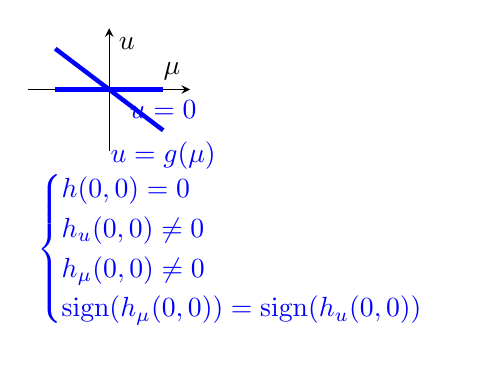
\begin{tikzpicture}
                  \begin{axis}[
                          width=0.3\textwidth,
                          axis lines = middle,
                          xlabel = $\mu$,
                          ylabel = {$u$},
                          xtick=\empty,
                          ytick=\empty,
                          domain=-1:1,
                          ymin = -1.5,
                          ymax = 1.5,
                          xmin = -1.5,
                          xmax = 1.5,
                          clip=false
                      ]
                      \addplot[blue, ultra thick] {0} node[below] {$u = 0$};
                      \addplot[blue, ultra thick] {-x} node[below] {$u = g(\mu)$};
                  \end{axis}
                  \node[blue] at (2.75, -1.25) {$\begin{cases}
                              h(0, 0) = 0          \\
                              h_u(0, 0) \neq 0     \\
                              h_{\mu}(0, 0) \neq 0 \\
                              \text{sign}(h_{\mu}(0, 0)) = \text{sign}(h_u(0, 0))
                          \end{cases}$};
              \end{tikzpicture}
              \hspace{1cm}
              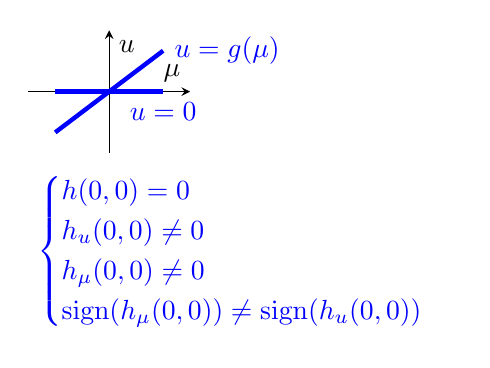
\begin{tikzpicture}
                  \begin{axis}[
                          width=0.3\textwidth,
                          axis lines = middle,
                          xlabel = $\mu$,
                          ylabel = {$u$},
                          xtick=\empty,
                          ytick=\empty,
                          domain=-1:1,
                          ymin = -1.5,
                          ymax = 1.5,
                          xmin = -1.5,
                          xmax = 1.5,
                          clip=false
                      ]
                      \addplot[blue, ultra thick] {0} node[below] {$u = 0$};
                      \addplot[blue, ultra thick] {x} node[right] {$u = g(\mu)$};
                  \end{axis}
                  \node[blue] at (2.75, -1.25) {$\begin{cases}
                              h(0, 0) = 0          \\
                              h_u(0, 0) \neq 0     \\
                              h_{\mu}(0, 0) \neq 0 \\
                              \text{sign}(h_{\mu}(0, 0)) \neq \text{sign}(h_u(0, 0))
                          \end{cases}$};
              \end{tikzpicture}
          \end{center}

          CASE 1B. Assume instead $h_{\mu}(0, 0) = 0$.

          Now, $g'(0) = 0$ and the Taylor Expansion near $\mu = 0$ is
          \[g(\mu) = g(0) + g'(0) \mu + O(\mu^2) \approx 0\]
          so we have
          \begin{center}
              \color{black}
              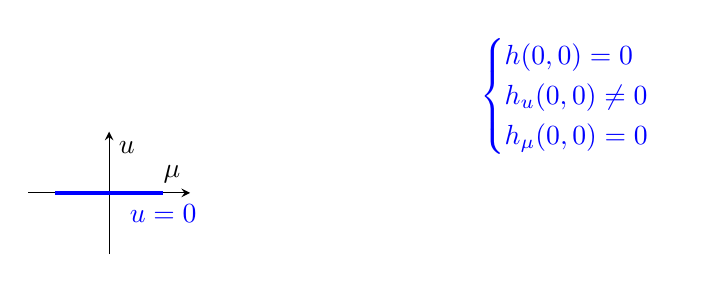
\begin{tikzpicture}
                  \begin{axis}[
                          width=0.3\textwidth,
                          axis lines = middle,
                          xlabel = $\mu$,
                          ylabel = {$u$},
                          xtick=\empty,
                          ytick=\empty,
                          domain=-1:1,
                          ymin = -1.5,
                          ymax = 1.5,
                          xmin = -1.5,
                          xmax = 1.5,
                          clip=false
                      ]
                      \addplot[blue, ultra thick] {0} node[below] {$u = 0$};
                  \end{axis}
                  \node[blue] at (7, 2) {$\begin{cases}
                              h(0, 0) = 0       \\
                              h_u(0, 0) \neq 0  \\
                              h_{\mu}(0, 0) = 0 \\
                          \end{cases}$};
              \end{tikzpicture}
          \end{center}

          CASE 2. Rather than letting $h_u(0, 0) \neq 0$, suppose $h_u(0, 0) = 0$.

          Now, just apply the IFT to the other variable to get $\mu = g(u)$ and
          \begin{gather*}
              h_u(u, g(u)) + h_{\mu}(u, g(u)) g'(0) = 0\\
              h_u(0, 0) + h_{\mu}(0, 0) g'(0) = 0\\
              h_{\mu}(0, 0) g'(0) = 0
          \end{gather*}

          But assuming $h_{\mu}(0, 0) = 0$,
          \[g(u) = g(0) + g'(0)u + O(u^2) = 0\]
          and we get the bifurcation diagram

          \begin{center}
              \color{black}
              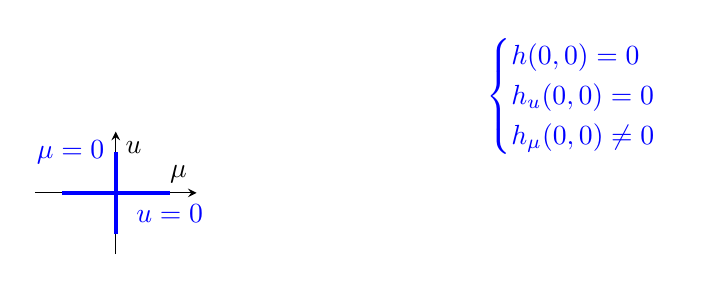
\begin{tikzpicture}
                  \begin{axis}[
                          width=0.3\textwidth,
                          axis lines = middle,
                          xlabel = $\mu$,
                          ylabel = {$u$},
                          xtick=\empty,
                          ytick=\empty,
                          domain=-1:1,
                          ymin = -1.5,
                          ymax = 1.5,
                          xmin = -1.5,
                          xmax = 1.5,
                          clip=false
                      ]
                      \addplot[blue, ultra thick] ({0}, {x}) node[left] {$\mu = 0$};
                      \addplot[blue, ultra thick] {0} node[below] {$u = 0$};

                  \end{axis}
                  \node[blue] at (7, 2) {$\begin{cases}
                              h(0, 0) = 0          \\
                              h_u(0, 0) = 0        \\
                              h_{\mu}(0, 0) \neq 0 \\
                          \end{cases}$};
              \end{tikzpicture}
          \end{center}

          If, instead, both $h_u(0, 0) = 0$ and $h_{\mu}(0, 0) = 0$, then we would need to consider higher order terms.
          \color{black}

\end{enumerate}
\pagebreak

\section{Checking the conditions for saddle-node bifurcations}
Show that the differential equation
\[\frac{du}{dt} = \sin \mu+ (1+ \mu) u \sin u - u^3 e^u \]
udergoes a saddle-node bifurcation at $(u, \mu) = (0, 0)$. Sketch the resulting bifurcation diagram and indicate the stability of the equilibria in the $(\mu, u)$-plane near $(0, 0)$.

Hint: Use the results we derived in class

\color{blue}
Let $f(u, \mu) = \sin \mu+ (1+ \mu) u \sin u - u^3 e^u$. It suffices to show
\[\begin{cases}
        f(0, 0) =0           \\
        f_u(0, 0 ) = 0       \\
        f_{uu}(0, 0) \neq 0  \\
        f_{\mu}(0, 0) \neq 0 \\
    \end{cases}\]

Consider:
\begin{align*}
    f_u(u, \mu)     & = (1 + \mu) \sin u + (1 + \mu)u \cos u - 3u^2 e^u - u^3 e^u  \\
    f_{uu}(u, \mu)  & = 2(1 + \mu) \cos u + (1 + \mu)u \sin u - ue^u(u^2 + 6u + 6) \\
    f_{\mu}(u, \mu) & = \cos \mu + u \sin u
\end{align*}
So
\begin{align*}
    f(0, 0)       & = \sin 0 + (1 + 0)(0)s\in 0 - 0^3 e^0 = 0                             & \checkmark \\
    f_u(0, 0)     & = (1 + 0)\sin 0 + (1 + 0)(0)\cos 0 - 3(0)^2 e^0 - (0)^3 e^0 = 0       & \checkmark \\
    f_{uu}(0, 0)  & = 2(1 + 0)\cos 0 + (1 + 0)(0)\sin 0 - 0e^0(0^2 + 6(0) + 6) = 2 \neq 0 & \checkmark \\
    f_{\mu}(0, 0) & = \cos 0 + 0\sin 0 = 1 \neq 0                                         & \checkmark
\end{align*}

Hence, $(u, \mu) = (0, 0)$ is a saddle-node bifurcation.

By the Saddle-node bifurcation Theorem, $\exists g \in C^2$ with $f(u, \mu) = 0 \iff \mu = g(u)$ near $(0, 0)$. Further, $g(0) = 0$ and
\[g(u) = -\frac{1}{2} \frac{f_{uu}(0, 0)}{f_{\mu}(0, 0)}u^2 + O(u^3) = -\frac{1}{2} \cdot \frac{2}{1} \cdot u^2 = -u^2 + O(u^3)\]

Hence,
\[f_u(u, g(u)) = f_{uu}(0, 0)u + O(u^2) = 2u + O(u^2)\]
which means that $u$ is stable for $u < 0$ and unstable for $u > 0$.

\color{black}
\begin{center}
    \begin{tikzpicture}
        \begin{axis}[
                axis lines = middle,
                xlabel = $\mu$,
                ylabel = {$u$},
                xtick=\empty,
                ytick=\empty,
                ymin = -1.5,
                ymax = 1.5,
                xmin = -1.5,
                xmax = 1.5,
                clip=false
            ]
            \addplot[blue, dashed, domain=0:1] ({-x^2}, x);
            \addplot[blue, domain=-1:0] ({-x^2}, x);

        \end{axis}
        \node[blue, above] at (0, 0) {$\mu = g(u)$};

        \node[red] at (1.5, 1.5) {\rotatebox{180}{$\wedge$}};
        \node[red] at (2.5, 2) {\rotatebox{180}{$\wedge$}};
        \node[red] at (1.5, 0.5) {$\wedge$};
        \node[red] at (2.5, 1)   {$\wedge$};

        \node[red] at (1.5, 5) {$\wedge$};
        \node[red] at (2.5, 4.5) {$\wedge$};
        \node[red] at (1.5, 4) {\rotatebox{180}{$\wedge$}};
        \node[red] at (2.5, 3.5) {\rotatebox{180}{$\wedge$}};

        \node[red] at (4.5, 2) {\rotatebox{180}{$\wedge$}};
        \node[red] at (4.5, 1) {\rotatebox{180}{$\wedge$}};
        \node[red] at (6, 2) {\rotatebox{180}{$\wedge$}};
        \node[red] at (6, 1) {\rotatebox{180}{$\wedge$}};

        \node[red] at (4.5, 5) {$\wedge$};
        \node[red] at (4.5, 4) {$\wedge$};
        \node[red] at (6, 5)   {$\wedge$};
        \node[red] at (6, 4)   {$\wedge$};




    \end{tikzpicture}
\end{center}
\color{black}

\end{document}